\documentclass[14pt,a4paper]{scrartcl}
\usepackage[utf8]{inputenc}
\usepackage[english,russian, ukrainian]{babel}
\usepackage{misccorr, color, ragged2e, amsfonts, amsthm, graphicx, systeme, amsmath, mdframed, lipsum, setspace, mathtools, esint, color, listings}

\renewcommand\qedsymbol{$\blacksquare$}
\renewcommand*{\proofname}{\text{Доведення}}

\theoremstyle{definition}
\newtheorem*{defo}{Означення}
\newtheorem*{teo}{Теорема}
\newtheorem*{example}{Приклад}
\theoremstyle{remark}
\newtheorem*{remark}{Зауваження}
\theoremstyle{definition}
\newtheorem*{consequence}{Наслідок}
\theoremstyle{definition}
\newtheorem{statement}{Утверждение}[section]
\newmdtheoremenv{boxteo}{Теорема}[section]
\newtheorem*{look}{Позначення}

\setlength\parindent{0pt}

\DeclareMathOperator*\lowlim{\underline{lim}}
\DeclareMathOperator*\uplim{\overline{lim}}

\newcommand\independent{\protect\mathpalette{\protect\independenT}{\perp}}

\def\independenT#1#2{\mathrel{\rlap{$#1#2$}\mkern2mu{#1#2}}}

% Default fixed font does not support bold face
\DeclareFixedFont{\ttb}{T1}{txtt}{bx}{n}{12} % for bold
\DeclareFixedFont{\ttm}{T1}{txtt}{m}{n}{12}  % for normal

\definecolor{deepblue}{rgb}{0,0,0.5}
\definecolor{deepred}{rgb}{0.6,0,0}
\definecolor{deepgreen}{rgb}{0,0.5,0}

\doublespacing

\begin{document}

\def\be{\begin{equation}}
\def\ee{\end{equation}}

\def\bd{\begin{defo}}
\def\ed{\end{defo}}

\def\bbt{\begin{boxteo}}
\def\ebt{\end{boxteo}}

\def\i{\infty}
\def\d{\partial}

\def\vx{\overline{x}}
\def\vphi{\overline{\varphi}}
\def\vf{\overline{f}}

\begin{titlepage}
\begin{center}

\vspace*{0.1cm}
\vfill

{\huge \textbf{ТЕОРІЯ СТІЙКОСТІ}}\\
\vspace{5cm}
За лекціями Горбань Н.\\
\vspace{1cm}
Редактори: Терещенко Д.\\ \hspace{3.7cm} Людомирський Ю.

\vfill

2021

\end{center}
\end{titlepage}


\tableofcontents
\newpage

\section{Лекція 1}
\subsection{Нормальні системи диференційних рівнянь}


\be
\left\lbrace
\begin{gathered}
    x'_1 (t) = f_1(t, x_1 (t), ... , x_n(t)) \\
    x'_2 (t) = f_2(t, x_1 (t), ... , x_n(t)) \\
    \vdots \\
    x'_n (t) = f_n(t, x_1 (t), ... , x_n(t)) \\
\end{gathered}\right.
\ee

 Системою диф. рівнянь n-го порядку в нормальній формі називається система вигляду (1), де $ f_i : D \to \mathbb{R}, \quad D \subset \mathbb{R}^{n+1 }, \quad i = \overline{1, n}$.
\look
\[
      \overline{x}(t) = \left[\begin{array}{l}
      x_1(t)    \\
      \dots     \\
      x_n(t)
      \end{array}\right] \text{-- невідома вектор-функція}, \quad
      \overline{f}(t, \overline{x}(t)) = \left[\begin{array}{l}
      f_1     \\
      \dots  \\
      f_n
      \end{array}\right] \text{, що}
\]
$D \rightarrow \mathbb{R}, \quad D \subset \mathbb{R}^{n+1}$, тоді $(1): \overline{x}'(t) = \overline{f}(t, \overline{x}(t))$.


\def\rect{\textbf{П}}
\bd
\textbf{Розв'язком системи} (1) на $(\alpha , \beta)$ називається така вектор-функція $\overline{x} (t) \in C^1(\alpha , \beta)$, що:
\begin{enumerate}
  \item $(t, x_1(t), \dots, x_n(t)) \in D \quad \forall t \in (\alpha, \beta)$;
  \item $\overline{x}(t)$  перетворює $(1)$ на тотожність на інтервалі $(\alpha, \beta)$.
\end{enumerate}

\textbf{Загальним розв'язком системи}  (1) називається n-параметрична сім'я розв'язків (1), що охоплює всі розв'язки системи.
\ed

Задача Коші. Для заданих $t_0, \overline{x}^{0} \in D$ знайти такий розв'язок (1), що $\overline{x} (t_0) = \overline{x}^{0}$.
Нехай $\Pi = \{(t, \overline{x}) \in \mathbb{R} \quad \big| \quad |t-t_0| \leq a, \quad ||\overline{x} - \overline{x}_0|| \leq b \}$.

\begin{boxteo}[Теорема Пеано]
Нехай $\vec{f} \in C(\Pi)$. Тоді розв'язок задачі Коші:
\begin{gather*}
  \begin{cases}
    \overline{x}' = \overline{f}(t, \overline{x}) \\
    \overline{x}(t_0) = \overline{x}_0
  \end{cases}
\end{gather*}
існує принаймні на проміжку $I_h = (t_0 - h, t_0 + h)$, де $h = \min\{{a, \dfrac{b}{M}}\}$, \\ $M = \max\limits_{(t, x) \in \Pi} {||\overline{f}(t, \overline{x})||}$.
\end{boxteo}

\begin{boxteo}[про продовження]
Нехай для системи (1) виконується, що $\overline{f} \in C(D), \quad D \subset \mathbb{R}^{n + 1}$ -- обмежена область. Тоді $\forall t : (t_0, \overline{x}_0) \in D$ існують такі $t^{-}, t^{+} : t^{-} < t_0 < t^{+}$, що розв'язок системи (1) з початкової умови $\overline{x}(t_0) = \overline{x}_0$ існує на інтервалі $(t^{-}, t^{+})$, причому $(t^{-}, \overline{x}(t^{-})) \text{ та } (t^{+}, \overline{x}(t^{+}))$ належать межі області $D$.
    \begin{center} 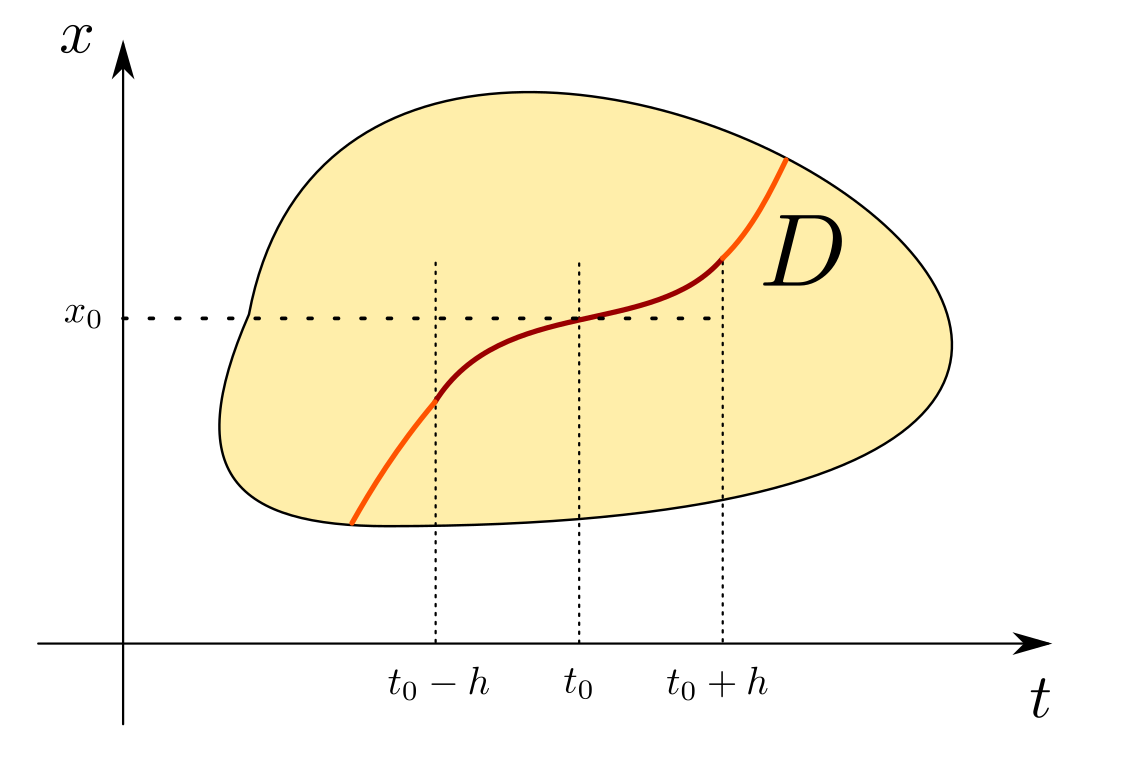
\includegraphics[scale=0.35]{assets/lect0.png} \end{center}
\end{boxteo}

\begin{boxteo}[Теорема Пікара]
  Нехай
  \begin{spacing}{1}
  \begin{enumerate}
    \item $\overline{f} \in C(\Pi)$;
    \item $\exists! L > 0 : \forall (t_1, \overline{x}_1), (t_2, \overline{x}_2) \in \Pi$ справедливо, що $|| f(t_1, \overline{x}_1) - f(t_2, \overline{x}_2)|| \leq \\ \leq L||\overline{x}_1 - \overline{x}_2||$ (умова Ліпшиця).
  \end{enumerate}
  \end{spacing}


  Тоді $\exists!$ розв'язок задачі Коші з початкової умови $\overline{x}(t_0) = \overline{x}_0(t)$, визначений принаймні на $I_h = (t_0 - h, t_0 + h), \quad h = \min\{{a, \dfrac{b}{M}}\}, \quad M = \max\limits_{\Pi}||f(t, \overline{x})||$.
\end{boxteo}

\subsection{Основні поняття теорії стійкості.}
Розглянем систему диференційних рівнянь $\overline{x}' = \overline{f}(t, \overline{x})$ (1), де $f : D \rightarrow \mathbb{R}^n$ та $D = [a, +\infty] \times G, \quad G \subset \mathbb{R}^n$. Нехай при цьому $\overline{f}$ задавольняє умовам існування та єдиності розв'язку задачі Коші в будь-якій точці $(t_0, \overline{x}_0) \in D$

\bd
Розв'язок $\overline{x} = \overline{\varphi}(t)$ системи (1) називається \textbf{стійким} за Ляпуновим, якщо

\begin{enumerate}
  \item $\overline{x} = \overline{\varphi}(t) \quad \exists  \text{ на } [a, +\infty]$ (відсутніть вертикальних асимптот)
  \item $\forall \varepsilon > 0 \quad \forall t_0 \geq a \quad \exists \delta > 0 : \forall $ розв'язку $\overline{x}(t)$ системи (1) такого, що $||\overline{x}(t_0) - \overline{\varphi}(t_0)|| < \delta$ виконується наступне, що $\overline{x}(t)$ існує на $[t_0, +\infty]$ та $||\overline{x}(t) - \overline{\varphi}(t)|| < \varepsilon \quad \forall t \geq t_0$.
\end{enumerate}
\ed

\begin{center} 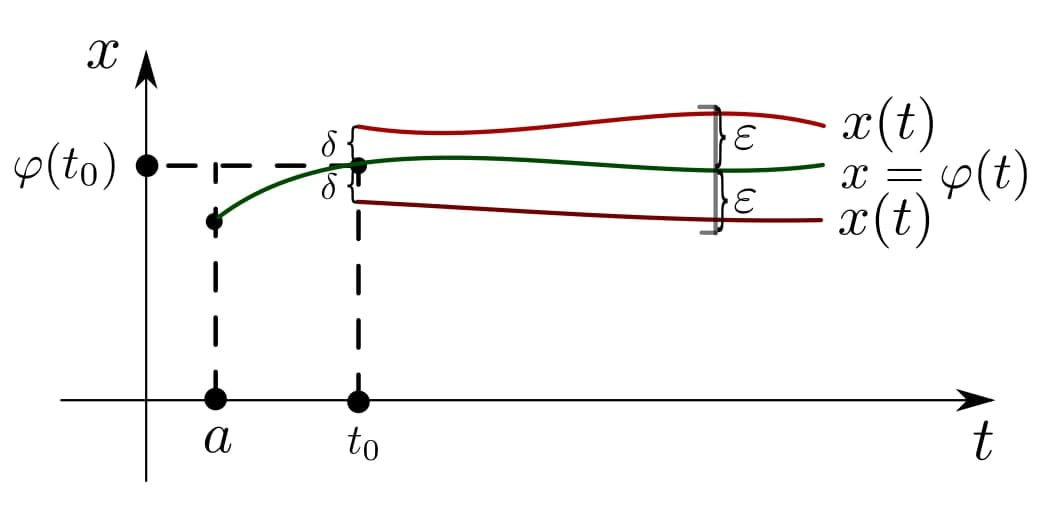
\includegraphics[scale=0.35]{assets/lect1.jpg} \end{center}

\bd
Розв'язок $\overline{x} = \overline{\varphi}(t)$ системи (1) називається \textbf{асимптотично стійким} за Ляпуновим, якщо

\begin{enumerate}
  \item $\overline{x} = \overline{\varphi}(t)$ стійкий;
  \item $\forall t_0 \geq a \quad \exists \delta > 0: \forall$ розв'язку $\vec{x}(t)$ с-ми (1) такого, що $||\vec{x}(t_0) - \vec{\varphi}(t_0)|| < \delta$ справедливо, що $||\vec{x}(t_0) - \vec{\varphi}(t_0)|| \rightarrow 0 \text{ при } t \rightarrow + \infty$.
\end{enumerate}

\begin{center} 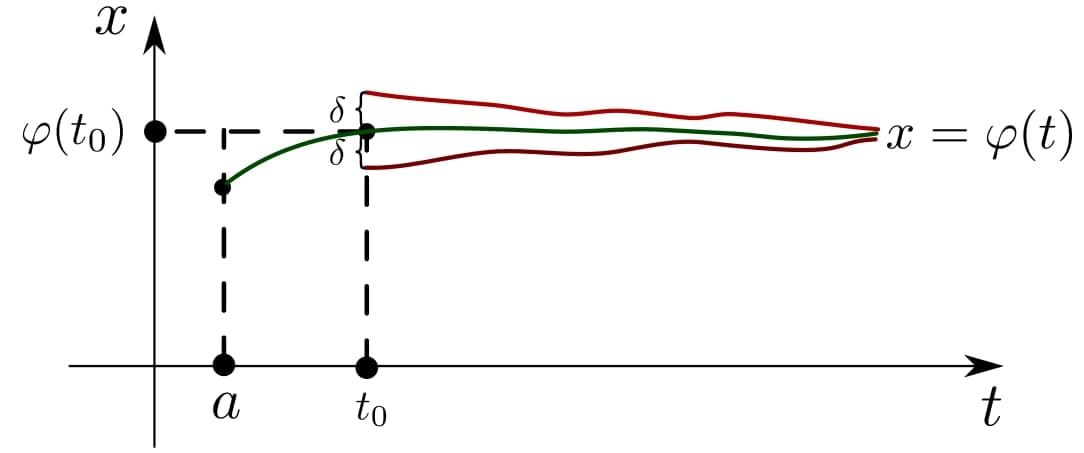
\includegraphics[scale=0.35]{assets/lect2.jpg} \end{center}

Роз'язок $\vec{\varphi}(t)$ називається \textbf{нестійким за Ляпуновим}, якщо він не є стійким, тобто:
\ed

\begin{enumerate}
  \item Або $\overline{x} = \overline{\varphi}(t) \quad \nexists$ на  $[a, +\infty]$ (вертикальні асимптоти);
  \item Або $\exists \varepsilon > 0 : \exists t_0 \geq a :  \forall \delta > 0$ існує розв'язок $\vec{x}(t)$ системи (1) такий, що $||\vec{x}(t_0) - \vec{\varphi}(t_0)|| < \delta$, але $||\vec{x}(t_0) - \vec{\varphi}(t_0)|| > \varepsilon$
\end{enumerate}

\begin{center} 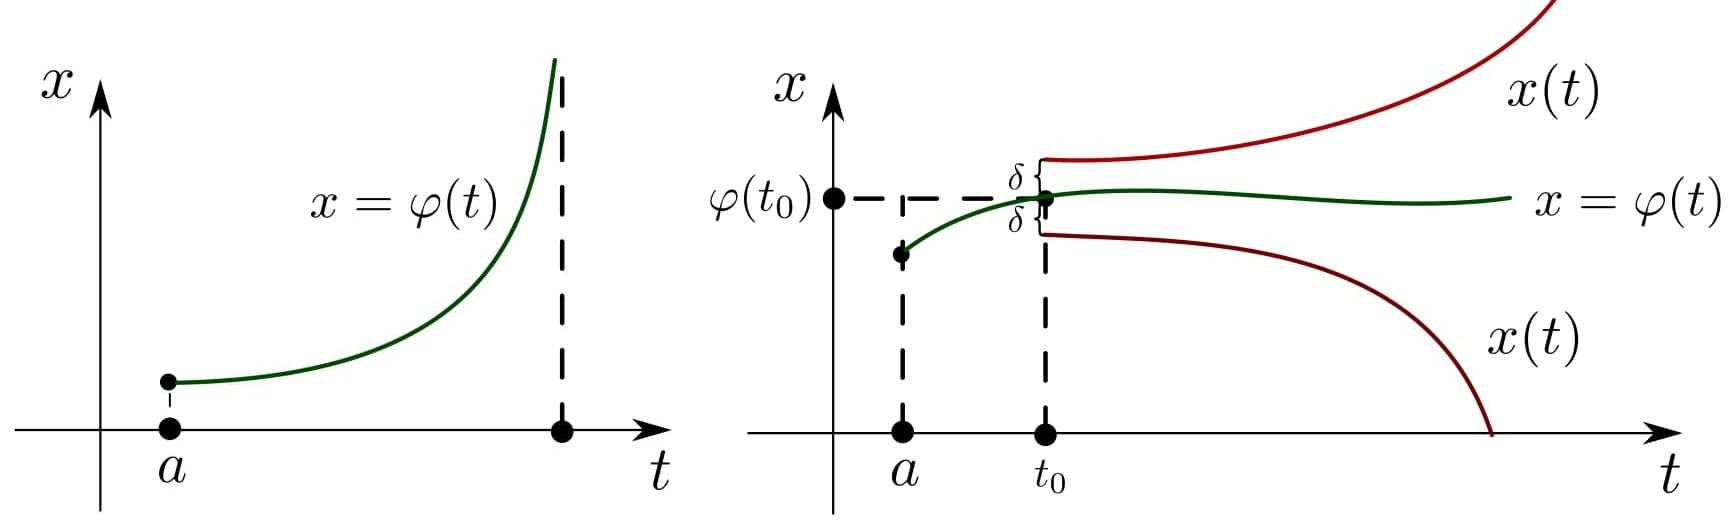
\includegraphics[scale=1.25]{assets/lect3+4.jpg} \end{center}

\subsection{Приклади дослідження на стійкість за означенням.}

\begin{example}
    Дослідити на стійкість розв'язок З.К.:
$$
\begin{cases}
    x = 1 \\
    x(0) = 0
\end{cases}
$$
1. Знайдемо розв'язок заданої З.К.: $x = 1 \Rightarrow x = t + C$ - заг. розв.\\
Підставимо: $ 0 = 0 + C \Longrightarrow C = 0 \Longrightarrow $ \fbox{ $ \varphi(t) = t $} - будемо досліджувати.
Зазначений розв'язок не має вертикальних асимптот та існує на всьому $\mathbb{R}$.
2. Знайдемо розв'язок довільної З.К. $x(t_0) = x_0$.
$$
x_0 = t_0 + C \Rightarrow C = x_0 - t_0 \Rightarrow x(t) = t + x_0 - t_0
$$
3. Нехай $  \left| x(t_0) - \varphi(t_0) \right|  =  \left| x_0 - t_0 \right| < \delta  $ ;\\
Тоді $ \left| x (t) - \varphi (t) \right|  = \left|  x_0 - t_0 \right| < \varepsilon = \delta $.\\
Таким чином, розв'язок є стійким, але не є асимптотично стійким.

\end{example}

\begin{example}
    Дослідити на стійкість розв'язок З.К.:
    $$
    \begin{cases}
        \dot{x} = 1 + t - x \\
        x(0) = 0
    \end{cases}
    $$
    1. Знайдемо розв'язок даної задачі Коші:
    $$
    \dot{x} = - x + 1 + t = \left| \text{ методом Бернуллі } \right| = t + Ae^{-t}
    $$
    Знайшли загальний розв'язок. Підставимо умову із з. К.: $ A = 0 \Rightarrow \fbox {$\varphi(t) = t$ }$\\
    2. Знайдемо розв'язок довільної З.К.:
    $$
    x(t_0) = x_0 \qquad x_0 = t_0 + Ae^{-t_0} \qquad A = (x_0 - t_0) e^{t_0}
    $$
    $$
    x(t) = t + (x_0 - t_0) e^{t_0 - t} - \text{ загальний розв'язок з. К.}
    $$

    3. Нехай $ \left|  x(t_0) - \varphi(t_0)  \right| = \left| x_0 - t_0 \right|  < \delta $. Розглядаємо: $ \forall t \geq t_0 :$
    $$
    \left| x(t) - \varphi(t) \right| = \left| t + (x_0 - t_0) \cdot e^{ t_0 - t} - t \right| =
     \left| x_0 - t_0 \right|< \delta  \to 0  \quad (t \to + \infty)
    $$
    Отримали, що знайдений розв'язок є асимптотично стійким.
\end{example}
Перейдемо знов до систем диф. рівнянь: $ \vx' = \vf (t, \vx)  \quad (1)$.\\
$\vx = \vphi (t)$ - розв'язок, який ми маємо дослідити на стійкість.\\
Заміна $ \overline{z} (t) = \vx (t)  - \vphi (y) $. Отримаємо систему:
$$ \overline{z}' + \overline{\varphi}'  = \overline{f} (t, \overline{z}+ \overline{\varphi})(t)$$
$$
\overline{f}' (t) = \overline{f} (t, \overline{\varphi})  \Longrightarrow \fbox{ $ \overline{z} ' = \overline{\varphi} (t, \overline{z} + \overline{\varphi} (t)) - \overline{f} ( t, \varphi(t)) $}
$$

Sample



\end{document}
